\subsection{Μοντελοποίηση πρόωσης και πέδησης}

Για τη μοντελοποίηση της ροπής επιτάχυνσης και πέδησης, συχνά υλοποιείται μοντέλο
πλήρους δυναμικής των περιστρεφόμενων μαζών. Στην περίπτωσή μας όπου χρησιμοποιούμε
QSS μοντέλο, μπορούμε να προσεγγίσουμε και τους τροχούς σε συνθήκες μόνιμη κατάσταση.

\noindent
Επιπλέον, αναζητούμε τα φορτία του εκάστοτε τροχού με δεδομένο συνολικό φορτίο
οχήματος, όπως θα αναλυθεί και στο επόμενο κεφάλαιο.

\subsubsection{Μοντέλο πέδησης}
\label{subsubsec:brakingModel}

Η κατανομή της ροπής πέδησης σε ένα όχημα καθορίζεται από την υδραυλική πίεση του συστήματος πέδησης.
Σε αγωνιστικά οχήματα, όπου συνήθως δε χρησιμοποιούνται ηλεκτρονικές υποβοηθήσεις (ABS -- Anti-lock Brake System),
η πίεση στους δύο τροχούς κάθε άξονα είναι ίση, ενώ η κατανομή στον εμπρός και πίσω άξονα μπορεί να είναι διαφορετική.
Η κατανομή της ροπής πέδησης στους δύο άξονες (brake bias) ελέγχεται από τον λόγω των εμβαδών των εμβόλων στις δύο τρόμπες
φρένων (master cylinders), αλλά μπορεί να μεταβάλλεται και δυναμικά μέσω μίας ρυθμιζόμενης ράβδου (balance bar) (\cref{fig:balanceBar}).

\begin{figure}[ht!]
    \begin{center}
        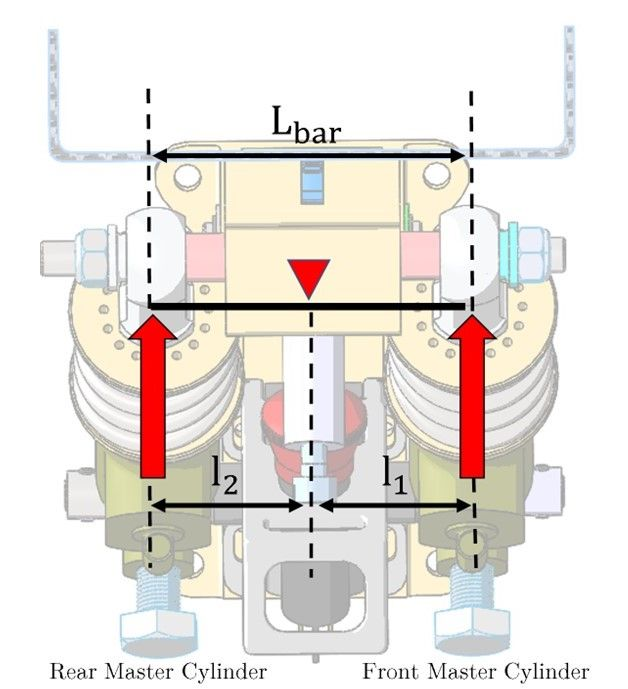
\includegraphics[width=0.6\textwidth]{figures/Balance_bar_scheme.jpg}
    \end{center}
    \caption{Σχηματική αναπαράσταση ρυθμιστικής ράβδου (balance bar) \cite{balanceBar}}
    \label{fig:balanceBar}
\end{figure}

Η εμπρόσθια κατανομή πέδησης μοντελοποιείται με μια μεταβλητή $k_{br,f}$ -- παράμετρο του οχήματος -- η οποία μοιράζει το απαιτούμενο
φορτίο πέδησης στους δύο άξονες και αντικατοπτρίζει τους παραπάνω μηχανισμούς. Η ροπή πέδησης θεωρείται πως ισομοιράζεται στους
δύο τροχούς ενός άξονα, με εξαίρεση την περίπτωση όπου ένας ασθενέστερος εκ των δύο χάνει πρώτος πρόσφυση (βλ. κεφάλαιο \ref{sec:inverseModel}).

\begin{equation}
    \begin{aligned}
        F_{x,br,f} &= k_{br,f}F_{x,br}\\
        F_{x,br,r} &= (1-k_{br,f})F_{x,br}
    \end{aligned}
    \label{eq:brakingDistribution}
\end{equation}

\subsubsection{Μοντέλο πρόωσης}

Στην παρούσα εργασία, θεωρείται πως θα αντιμετωπίζουμε οχήματα με κίνηση μόνο στον πίσω άξονα, ωστόσο σε άλλη περίπτωση (όπως λ.χ τετρακίνησης) θα μπορούσε να 
πραγματοποιηθεί με τη μοντελοποίηση ενός κεντρικού διαφορικού ή με μία σταθερή κατανομή όπως στην περίπτωση της πέδησης.\\[10pt]
\noindent
Επομένως, για τον πίσω άξονα, η κατανομή της δύναμης πρόωσης επιτυγχάνεται με ένα μοντέλο διαφορικού περιορισμένης ολίσθησης "μπλοκέ" (LSD -- Limited Slip Differential). 

\begin{equation}
    R\bigl(F_{L,rx} - F_{R,rx}\bigr) = -k_d\bigl(\omega_{L,r}-\omega_{R,r}\bigr)
    \label{eq:differential}
\end{equation}

Όπου,
\begin{itemize}
    \item $F_{L,rx}, F_{R,rx}$, οι δυνάμεις πρόωσης του αριστερού και δεξιού τροχού αντίστοιχα,
    \item $\omega_{L,r}, \omega_{R,r}$, οι γωνιακές ταχύτητες του αριστερού και δεξιού τροχού αντίστοιχα
    \item $k_d$, ένας συντελεστής στρεπτικής απόσβεσης (0 αντιστοιχεί σε ανοιχτό διαφορικό, και μεγάλες τιμές αντιστοιχούν σε "κλειδωμένο")
\end{itemize}

Καθώς το όχημα θεωρείται σε μόνιμη κατάσταση, οι γωνιακές ταχύτητες των τροχών προσεγγίζονται κινηματικά από τις εξισώσεις \ref{eq:wheelOmega}. Οι πραγματικές γωνιακές ταχύτητες θα πρέπει να διαφέρουν από τις κινηματικές ώστε να παράγουν δυνάμεις,
ωστόσο, ακόμη και με την κινηματική προσέγγιση, η διαφορά των δύο ταχυτήτων στην \cref{eq:differential} θα παραμένει περίπου ίδια.

\begin{equation}
    \begin{aligned}
        \omega_{L,r} &= U_x + \Bigl(r_{\text{καμπ.}}-\dfrac{t_r}{2}\Bigr)\dot{\psi}\\
        \omega_{R,r} &= U_x + \Bigl(r_{\text{καμπ.}}+\dfrac{t_r}{2}\Bigr)\dot{\psi}\\
    \end{aligned}
    \label{eq:wheelOmega}
\end{equation}

